\documentclass{standalone}
\usepackage{tikz}
\usepackage{amsmath}
\usetikzlibrary{arrows.meta, calc}

\begin{document}
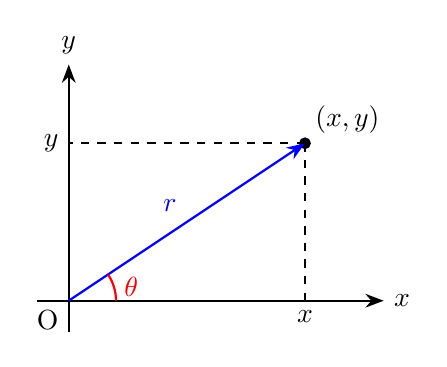
\begin{tikzpicture}[scale=2, thick, >=Stealth]

  % Axes
  \draw[->] (-0.2,0) -- (2,0) node[right] {$x$};
  \draw[->] (0,-0.2) -- (0,1.5) node[above] {$y$};

  % Coordinates
  \coordinate (O) at (0,0);    % origin
  \coordinate (P) at (1.5,1);  % point (x,y)
  \coordinate (X) at (P|-O);   % projection on x-axis
  \coordinate (Y) at (O|-P);   % projection on y-axis

  % Dashed projections
  \draw[dashed] (P) -- (X);
  \draw[dashed] (P) -- (Y);

  % Point
  \draw[fill=black] (P) circle (0.03) node[above right] {$(x, y)$};

  % Radius vector r
  \draw[->, blue, thick] (O) -- (P) node[midway, above left] {$r$};

  % Projection labels
  \node[below] at (X) {$x$};
  \node[left] at (Y) {$y$};
  \node[below left] at (O) {O};

  % Angle θ (hardcoded for compatibility: atan(1/1.5) ≈ 33.69 degrees)
  \def\angleTheta{33.69}
  \draw[red, thick] (0.3,0) arc (0:\angleTheta:0.3) node[midway, right] {$\theta$};

\end{tikzpicture}
\end{document}